\documentclass[tikz,border=6pt]{standalone}
\usepackage[scaled]{helvet}
\renewcommand{\familydefault}{\sfdefault}
\usetikzlibrary{arrows.meta,positioning,shapes.geometric}
\definecolor{ink}{HTML}{12343B}\definecolor{ice}{HTML}{DCEBF1}\definecolor{grey}{HTML}{EEF3F4}
\definecolor{good}{HTML}{DDEFE7}\definecolor{warn}{HTML}{F5EBCF}\definecolor{bad}{HTML}{F4D9D5}
\tikzset{
 q/.style={diamond,aspect=2.6,draw=ink,fill=ice,align=center,font=\small,inner sep=0pt,text width=37mm},
 s/.style={draw=ink,rounded corners=2pt,align=center,font=\small,fill=grey,text width=58mm,minimum height=10mm},
 a/.style={draw=ink,rounded corners=2pt,align=center,font=\small,text width=54mm,minimum height=10mm},
 arr/.style={-{Stealth[length=2.4mm]},draw=ink,thick}, l/.style={font=\scriptsize,midway,fill=white,inner sep=1pt}}
\begin{document}
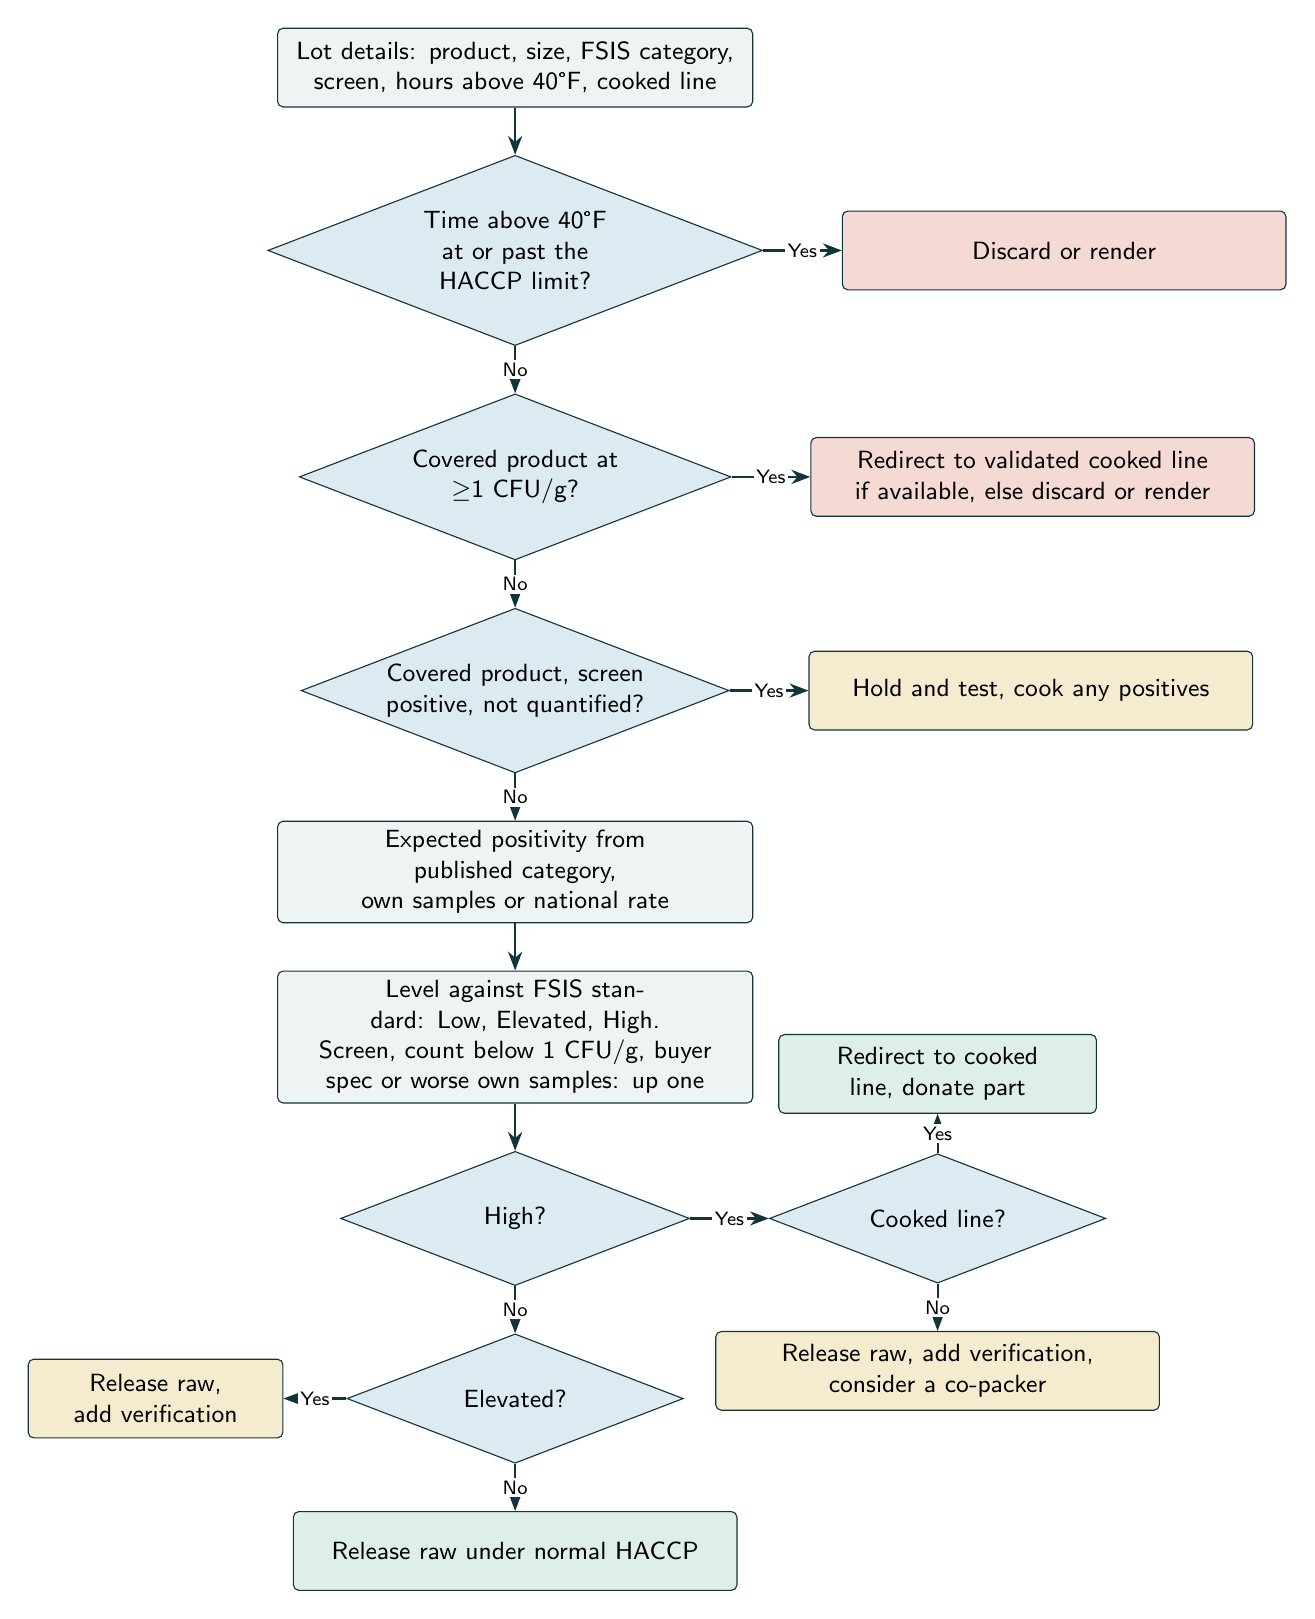
\begin{tikzpicture}[node distance=6mm and 10mm]
\node[s] (in) {Lot details: product, size, FSIS category,\\screen, hours above 40\textdegree F, cooked line};
\node[q,below=of in] (temp) {Time above 40\textdegree F\\at or past the HACCP limit?};
\node[q,below=of temp] (cov) {Covered product at\\$\geq$1 CFU/g?};
\node[q,below=of cov] (hold) {Covered product, screen\\positive, not quantified?};
\node[s,below=of hold] (rate) {Expected positivity from published category,\\own samples or national rate};
\node[s,below=of rate] (lvl) {Level against FSIS standard: Low, Elevated, High.\\Screen, count below 1 CFU/g, buyer spec or worse own samples: up one};
\node[q,below=of lvl] (high) {High?};
\node[a,fill=bad,right=of temp] (disc) {Discard or render};
\node[a,fill=bad,right=of cov] (red) {Redirect to validated cooked line\\if available, else discard or render};
\node[a,fill=warn,right=of hold] (ht) {Hold and test, cook any positives};
\node[q,right=of high] (line) {Cooked line?};
\node[a,fill=warn,below=of line] (ver2) {Release raw, add verification,\\consider a co-packer};
\node[a,fill=good,above=of line,yshift=-1mm,text width=38mm] (don) {Redirect to cooked line, donate part};
\node[q,below=of high] (el) {Elevated?};
\node[a,fill=warn,left=8mm of el,text width=30mm] (ver) {Release raw,\\add verification};
\node[a,fill=good,below=of el] (rel) {Release raw under normal HACCP};
\draw[arr] (in)--(temp);
\draw[arr] (temp)--node[l]{No}(cov);
\draw[arr] (cov)--node[l]{No}(hold);
\draw[arr] (hold)--node[l]{No}(rate);
\draw[arr] (rate)--(lvl);
\draw[arr] (lvl)--(high);
\draw[arr] (high)--node[l]{No}(el);
\draw[arr] (el)--node[l]{No}(rel);
\draw[arr] (el)--node[l]{Yes}(ver);
\draw[arr] (temp)--node[l]{Yes}(disc);
\draw[arr] (cov)--node[l]{Yes}(red);
\draw[arr] (hold)--node[l]{Yes}(ht);
\draw[arr] (high)--node[l]{Yes}(line);
\draw[arr] (line)--node[l]{Yes}(don);
\draw[arr] (line)--node[l]{No}(ver2);
\end{tikzpicture}
\end{document}
